\documentclass{beamer}
\usetheme{Boadilla}
\usepackage[utf8x]{inputenc}
\usepackage{listings}
\usepackage{subfig}
%\title{LS Genio Platform}
%\subtitle{Piattaforma per il monitoraggio di macchine utensili con integrazione a software ERP Microsoft Dynamics NAV}
%\author{Vincenzo Nucci e Matteo Tiberi}
%\author{Matteo Tiberi}
%\institute{Università di Camerino}
\date{}
\begin{document}
	
	\begin{frame}
	\centering
	
\includegraphics[scale=0.25]{images/frontespizio-beamer.png}\par
	\usebeamertemplate{title page}
\end{frame}

\begin{frame}
\frametitle{Obiettivi}
\begin{itemize}
	\item Sviluppo di una piattaforma indipendente
	\begin{itemize}
		\item Monitoraggio di macchine utensili
		\item PLC raccolgono dati dai sensori
		\item Integrazione tra applicazioni e PLC
	\end{itemize}
	\item Piattaforma come mash-up
	\begin{itemize}
		\item Diversi componenti integrati tra loro
	\end{itemize}
	%\item Servizio di sottoscrizione "subscribe"
	%\begin{itemize}
	%	\item Notifica dei messaggi PUSH
	%\end{itemize}
	%\item Integrazione dei servizi con NAV
	%\item Servizio di monitoraggio dei dati
	%\begin{itemize}
	%	\item Controllo valore oltre soglia
	%\end{itemize}
\end{itemize}
\end{frame}

\begin{frame}
\frametitle{LS Genio Mash-up}
\framesubtitle{Idea Architetturale}
%\textbf{Idea Architetturale} 
\begin{columns}[T] % align columns
	\begin{column}{.52\textwidth}
		\begin{itemize}
			\item Architettura orientata ai servizi REST
			\item Interfacce di comunicazione ben definite (JSON-ISO 19156:2011) 
			\item Subscribe per l'event listening (MOM ActiveMQ)
			\item Gestione della semantica delle misurazioni
			\item Architettura n-tier 
		\end{itemize}
	\end{column}%
	\hfill%
	\begin{column}{.48\textwidth}
		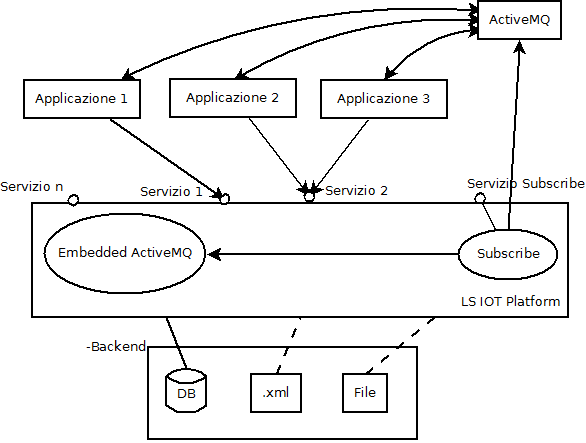
\includegraphics[width=0.9\textwidth]{images/architettura_piattaforma.png}
	\end{column}%
\end{columns}
\end{frame}

\begin{frame}
\frametitle{LS Genio Mash-up}
\framesubtitle{Interoperabilità tramite servizi REST}
\begin{columns}[T] % align columns
	\begin{column}{.4\textwidth}
		\begin{itemize}
			{\tiny
				\item API tramite servizi REST
				\item Servizi disponibili
				\begin{itemize}
					\tiny
					\item getlastmeasure
					\item getmeasurefromto
					\item getdetailedmeasurefromto
					\item getmeasurelastmonth
					\item getmeasurelastweek
					\item getdetailedmeasurelastmonth
					\item getdetailedmeasurelastweek
					\item getallplc
					\item sensordatafromfields
					\item subscribe
					\item unsubscribe
				\end{itemize}
			}
		\end{itemize}
		
	\end{column}%
	\hfill%
	\begin{column}{.56\textwidth}
		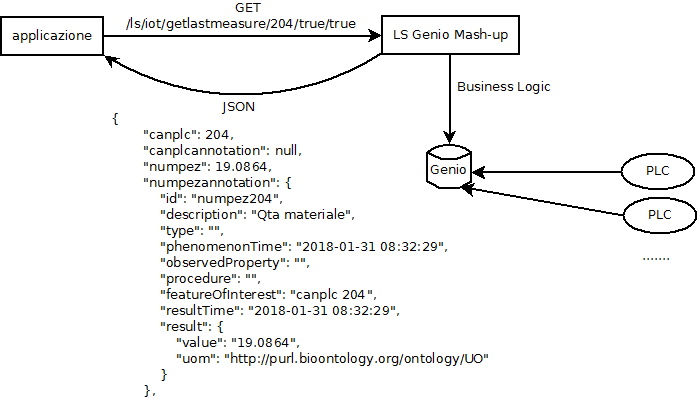
\includegraphics[width=1\textwidth]{images/interoperabilita-rest.png}
	\end{column}%
\end{columns}
\end{frame}

\begin{frame}
\frametitle{LS Genio Mash-up}
\framesubtitle{Schema servizio subscribe}
\begin{columns}[T] % align columns
	\begin{column}{.38\textwidth}
		\begin{itemize}
			\small
			\item Invio della regola di subscribe
			\item Un thread gestisce una regola
			\item Invio dei dati in ActiveMQ quando si verifica l'evento
			
		\end{itemize}
		
	\end{column}%
	\hfill%
	\begin{column}{.60\textwidth}
		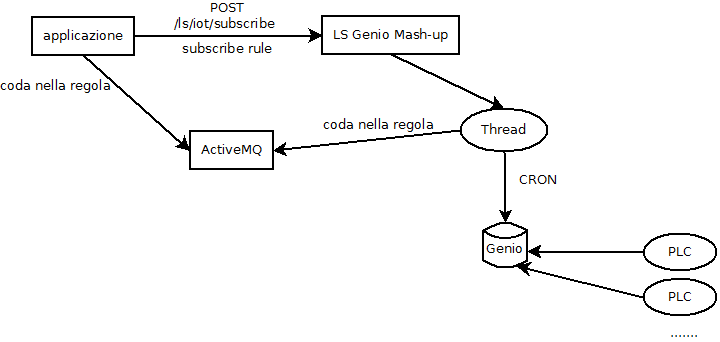
\includegraphics[width=1\textwidth]{images/schema-subscribe.png}
	\end{column}%
\end{columns}
\end{frame}

\begin{frame}
\frametitle{LS Genio Mash-up}
\framesubtitle{Gestione (GUI)}
\begin{columns}[T] % align columns
	\begin{column}{.3\textwidth}
		
		\begin{itemize}
			{\tiny
				\item \textbf{Interfaccia web catalogo Smart Object}
				
				\begin{itemize}
					{\tiny
						\item Permette agli utenti di informarsi sulle chiamate dei servizi
						\item Descrive la misura rappresentata dai campi della tabella in Genio
					}
				\end{itemize}
				
				%\item Interfaccia web gestione richieste
				%\item Interfaccia web gestione servizi utenti
				%\item Interfaccia web per il real time monitoring
				%\item Interfaccia web per la gestione della soglia
			}
		\end{itemize}
		
	\end{column}%
	\hfill%
	\begin{column}{.66\textwidth}
		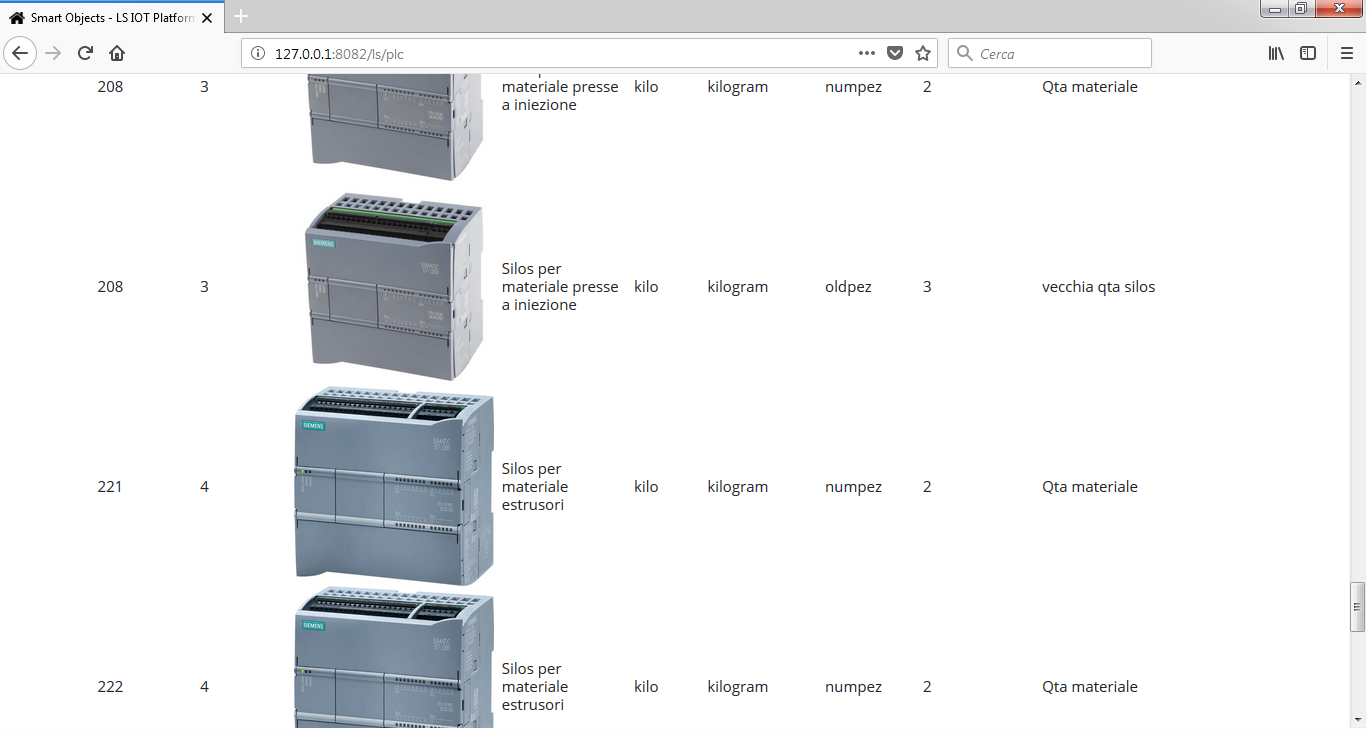
\includegraphics[width=0.9\textwidth]{images/SmartObjectsPlatform.png}
	\end{column}%
\end{columns}
\end{frame}

\begin{frame}
\frametitle{Streaming data visualization}
\framesubtitle{Interfaccia web per il real time monitoring}
\begin{columns}[T] % align columns
	\begin{column}{.3\textwidth}
		\begin{itemize}
			\small
			\item I dati che hanno una annotazione associata possono essere visualizzati
			\item PLC e campo come parametri di selezione
			\item Possibilità di avviare il controllo della soglia
		\end{itemize}
	\end{column}%
	\hfill%
	\begin{column}{.66\textwidth}
		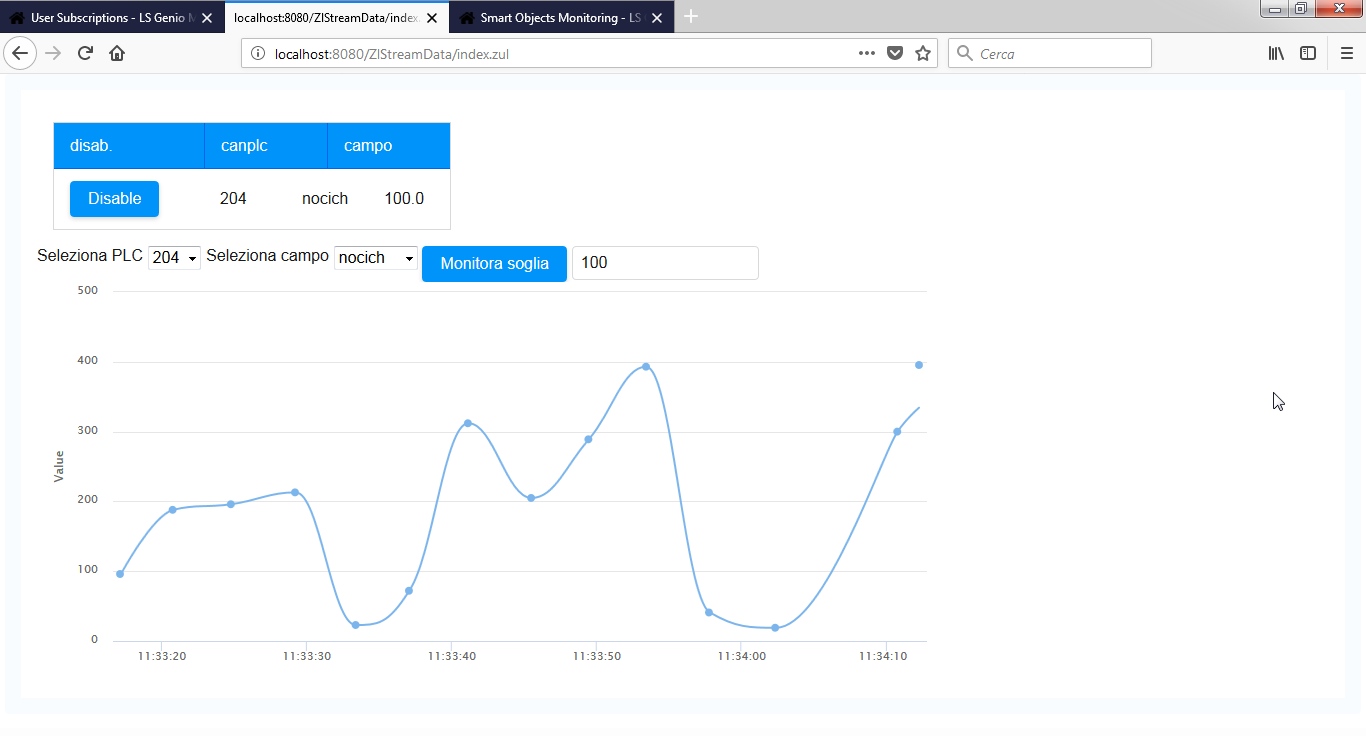
\includegraphics[width=1\textwidth]{images/grafico-zk.png}
	\end{column}%
\end{columns}

\end{frame}

\begin{frame}
	\frametitle{Conclusioni}
	Questo progetto ha mostrato quanta innovazione e benefici porti alle aziende implementare i concetti introdotti dall’Industria 4.0, tra i quali sono le componenti principali l'IoT e i Big Data. La possibilità di monitorare l'andamento dei macchinari in produzione non solo aumenta l'efficienza del processo produttivo ma aumenta anche la qualità del prodotto finale.
\end{frame}

%-------------------------inizio client-----------------------------
%\begin{frame}
%\frametitle{Sommario}
%La parte client è principalmente focalizzata sull’utilizzo dei servizi forniti dalla piattaforma LS-Genio Mashup con il software gestionale Microsoft Dynamics NAV e nella realizzazione di un ontologia delle misurazioni e misure dei dati restituiti (i quali sono relativi a misurazioni di sensori su macchine utensili). Su questi dati, inoltre, è stata realizzata una visualizzazione grafica visibile tramite il gestionale NAV.
%\end{frame}

\begin{frame}
\frametitle{Obiettivi}
\begin{itemize}
	\item Interazione di Microsoft Dynamics NAV con la piattaforma LS Genio Mash-up e definizione di un "setup" per l'utente
	%\item Interazione di Microsoft Dynamics NAV con la piattaforma LS-Genio Mashup
	%\begin{itemize}
	%	\item Definizione di un "setup"
	%	\item Rappresentazione grafica dei dati ottenuti
	%\end{itemize}
	
	%\item Visualizzazione tramite NAV di un report PowerBI basato sui dati ottenuti
	%\item Visualizzazione da NAV di una rappresentazione grafica con PowerBI dei dati ottenuti 
	\item Realizzazione di un ontologia delle misurazioni e delle misure
\end{itemize}	
\end{frame}

\begin{frame}
\frametitle{La pagina Machine Assignment List}
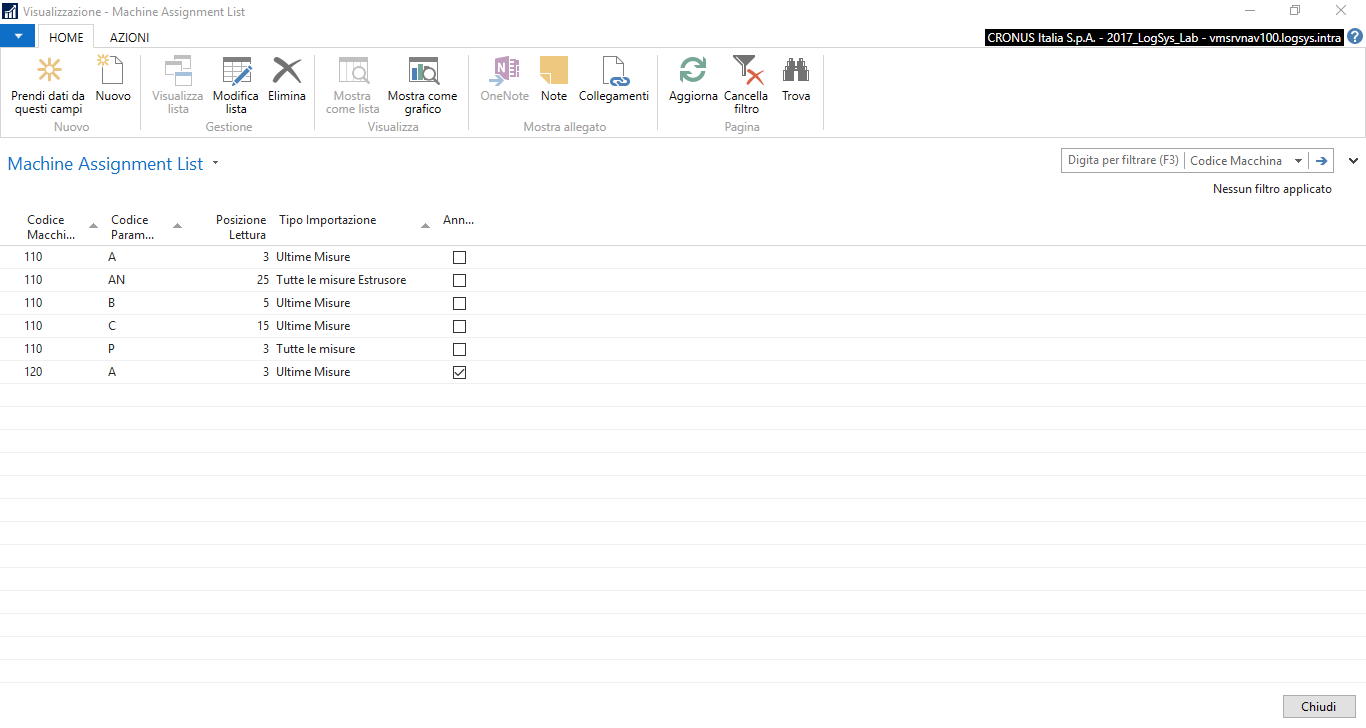
\includegraphics[width=1\textwidth]{images/MachineAssignmentList2.png}
\end{frame}


%\begin{frame}
%\frametitle{Lista con i parametri}
%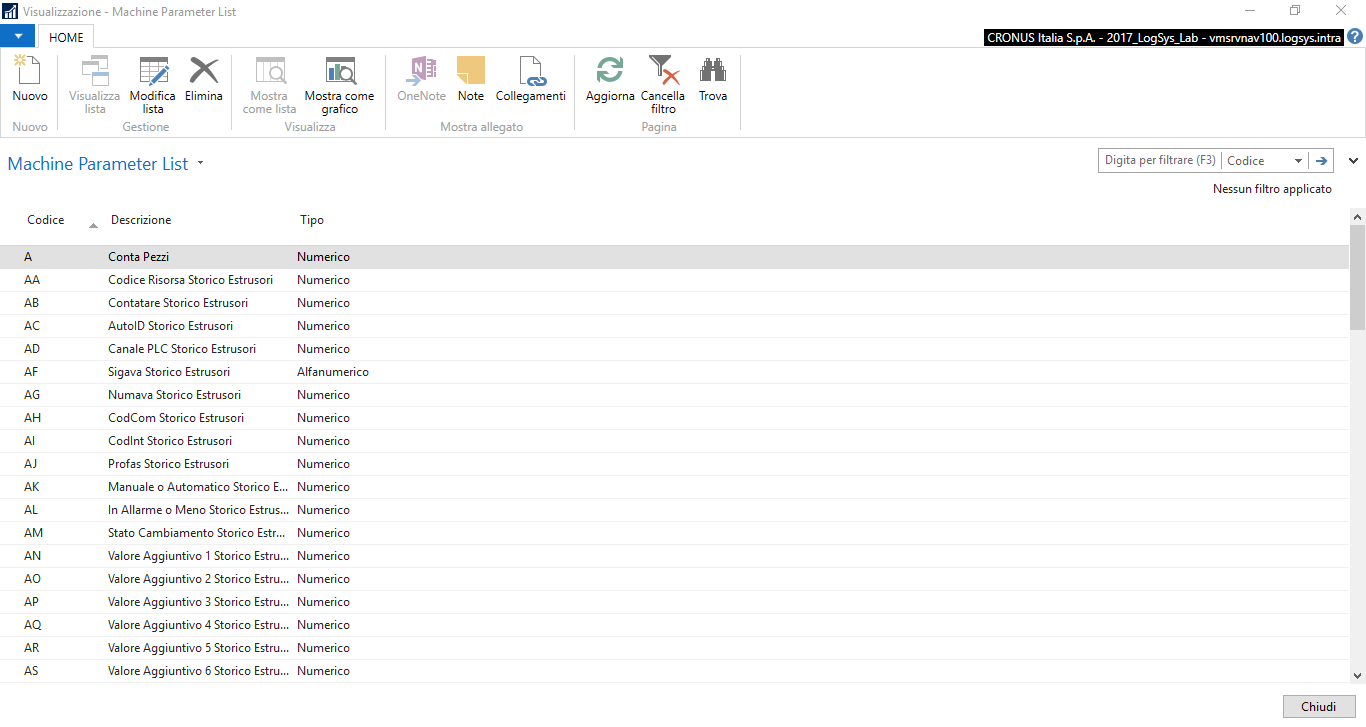
\includegraphics[width=1\textwidth]{images/MachineParameter.png}
%\end{frame}

%\begin{frame}
%\frametitle{Pagina del token}
%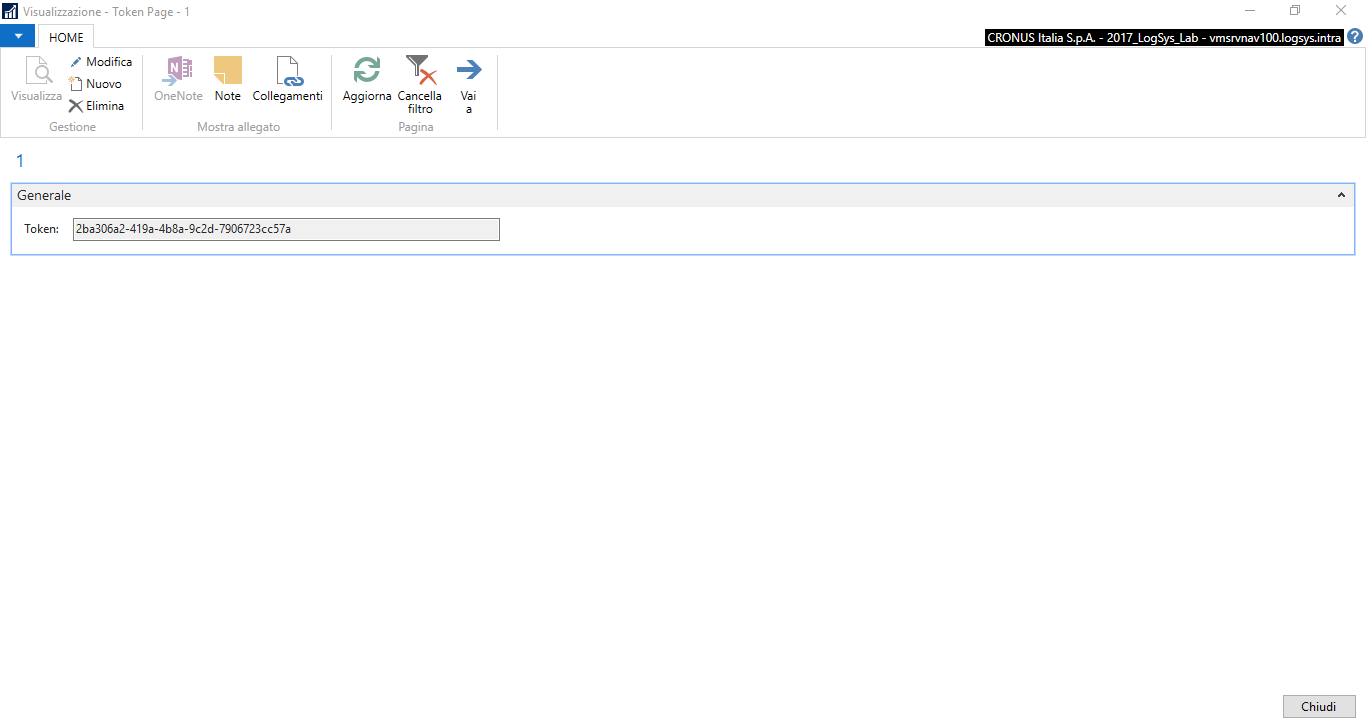
\includegraphics[width=1\textwidth]{images/tokenpage.png}
%\end{frame}



\begin{frame}
\frametitle{La pagina Machine Reading List}
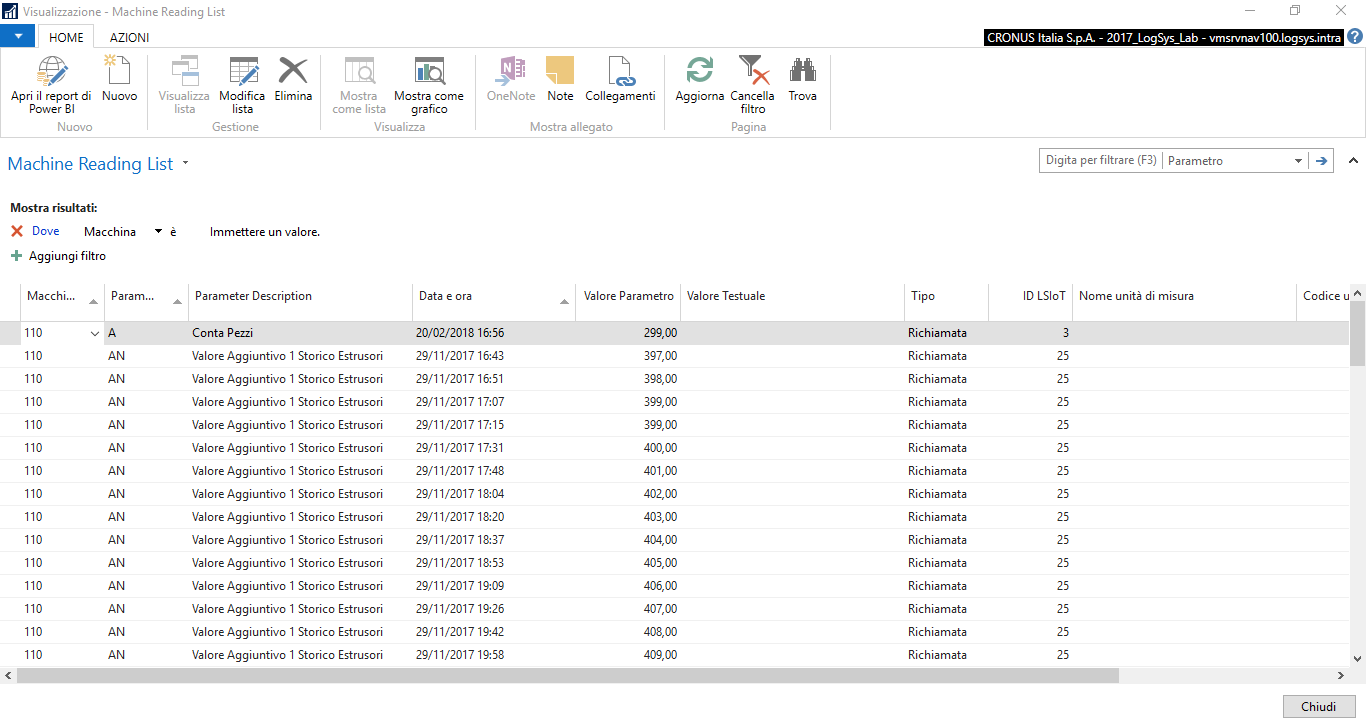
\includegraphics[width=1\textwidth]{images/MachineReadingList.png}
\end{frame}

%\begin{frame}
%\frametitle{Il report PowerBI nell'applicativo}
%\includegraphics[width=1\textwidth]{images/PowerBI.png}
%\end{frame}

\begin{frame}
\frametitle{Il report PowerBI esportato nel web}
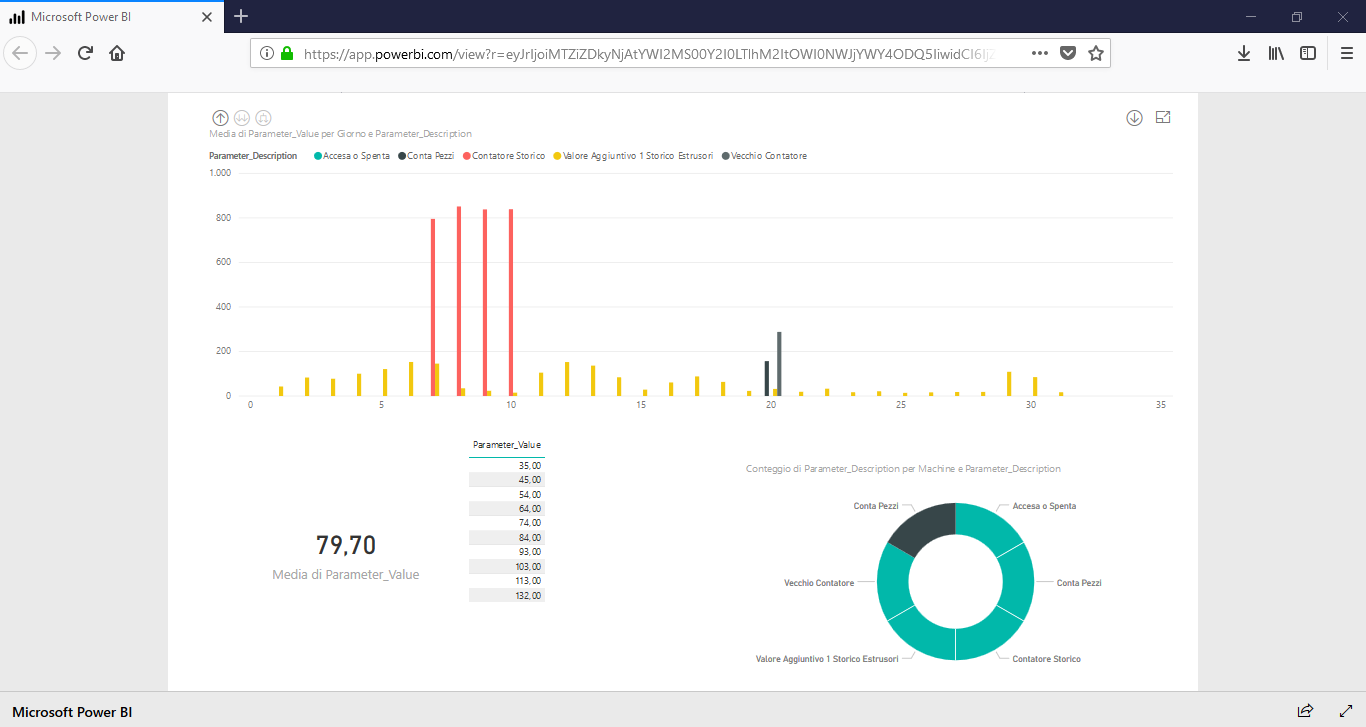
\includegraphics[width=1\textwidth]{images/ReportWEB.png}
\end{frame}

%\begin{frame}
%\frametitle{Metodo SetMeasurementPLC}
%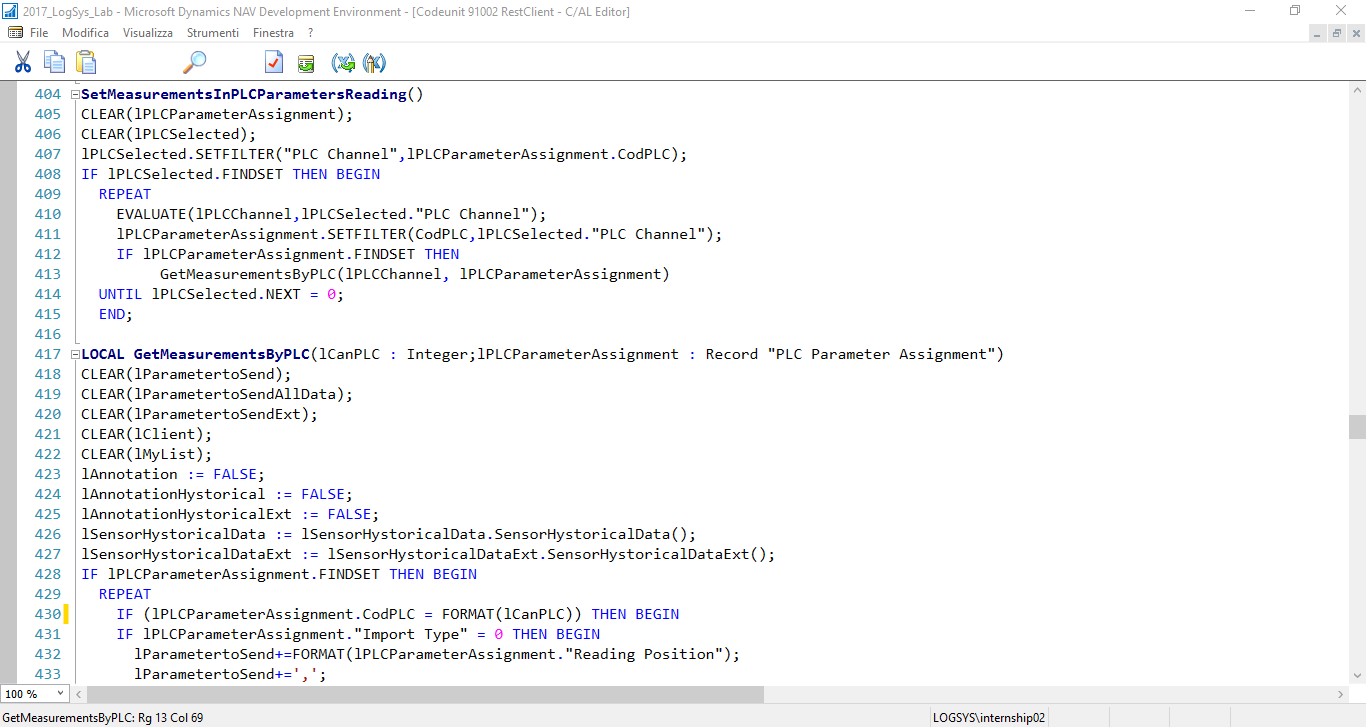
\includegraphics[width=1\textwidth]{images/NAVSetMesurament.png}
%\end{frame}

%\begin{frame}
%\frametitle{Metodo GetMeasurementPLC1}
%\includegraphics[width=1\textwidth]{images/NAVGetMesurament1.png}
%\end{frame}

%\begin{frame}
%\frametitle{Metodo GetMeasurementPLC2}
%\includegraphics[width=1\textwidth]{images/NAVGetMesurament2.png}
%\end{frame}

%\begin{frame}
%\frametitle{NAV servizi web}
%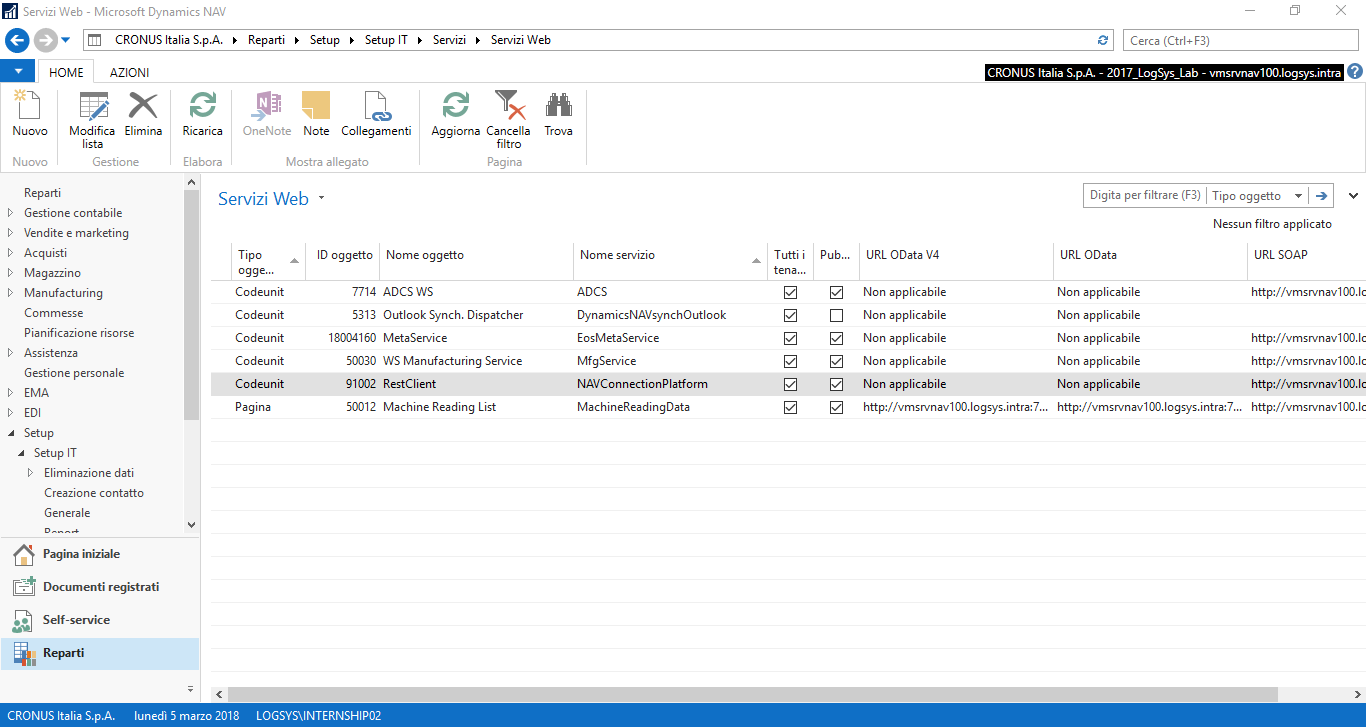
\includegraphics[width=1\textwidth]{images/NAVServiziWeb.png}
%\end{frame}


%\begin{frame}
%\frametitle{NAV SubscriptionPage}
%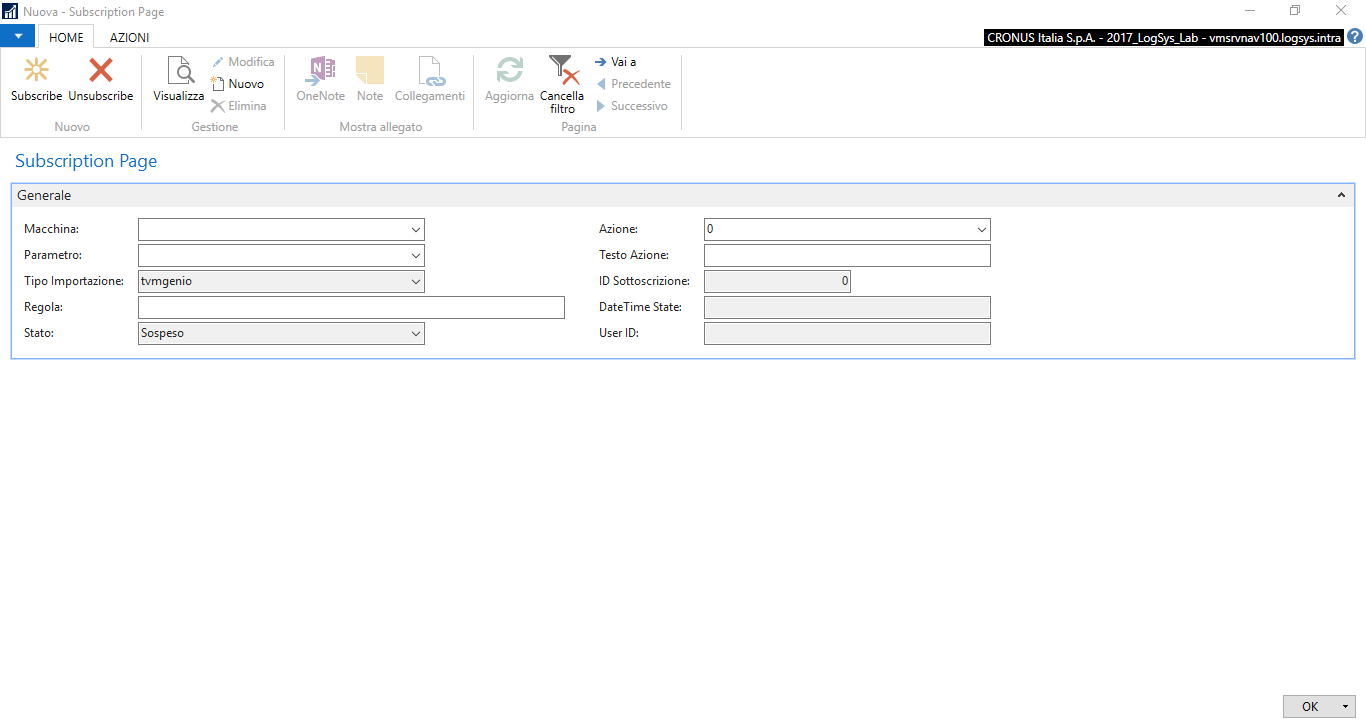
\includegraphics[width=1\textwidth]{images/NAVSubscriptionPage.png}
%\end{frame}



%\begin{frame}
%\frametitle{Tabelle Annotazioni}
%\includegraphics[width=1\textwidth]{images/AltreTabelleAnnotazioniMOD4.png}
%\end{frame}

%\begin{frame}
%\frametitle{Metodo PushMeasurement 1}
%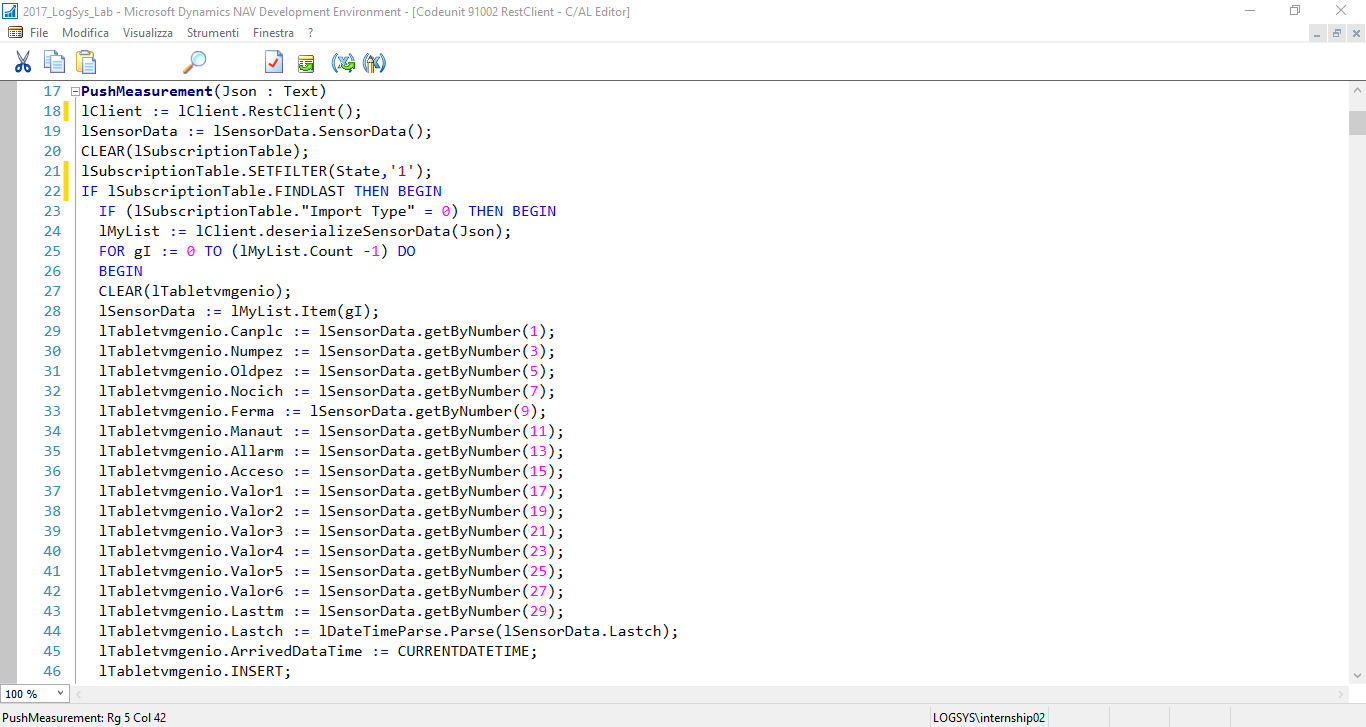
\includegraphics[width=1\textwidth]{images/NAVPushMeasuraments1.png}
%\end{frame}

%\begin{frame}
%\frametitle{Metodo PushMeasurement 2}
%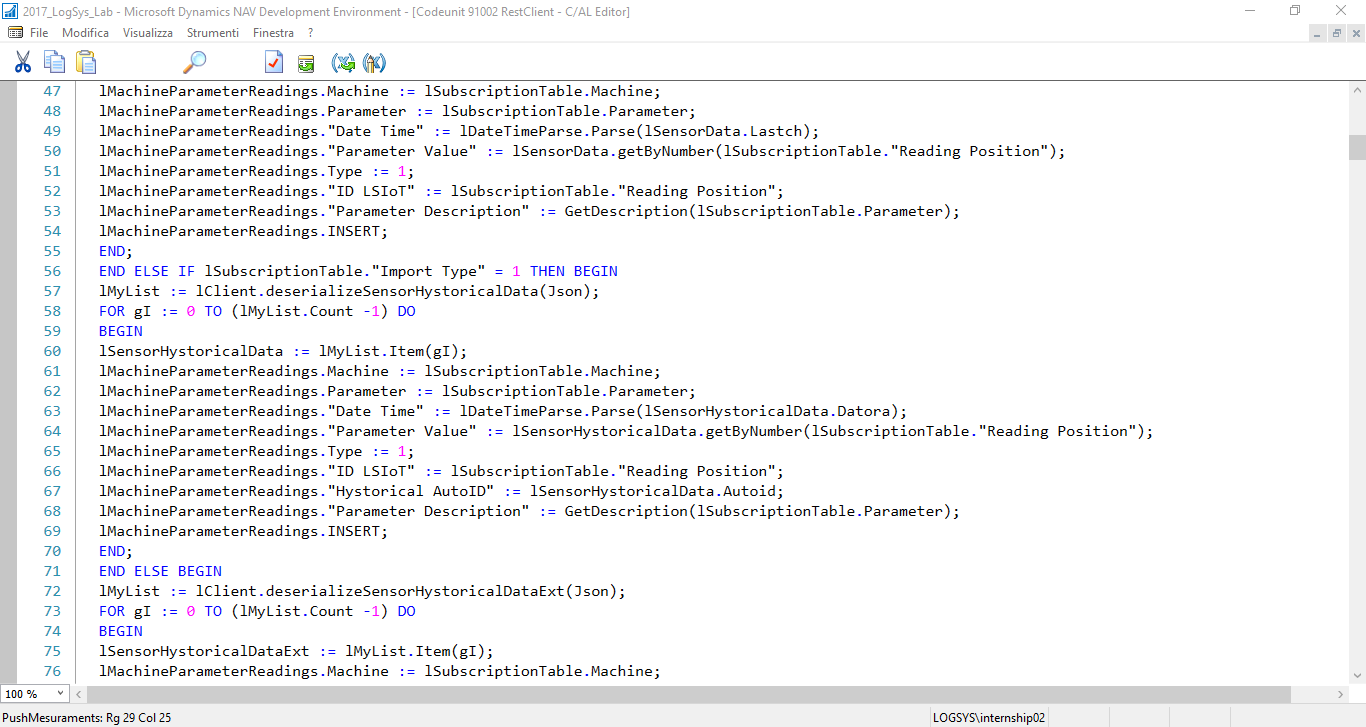
\includegraphics[width=1\textwidth]{images/NAVPushMeasuraments2.png}
%\end{frame}

%\begin{frame}
%\frametitle{Metodo PushMeasurement 3}
%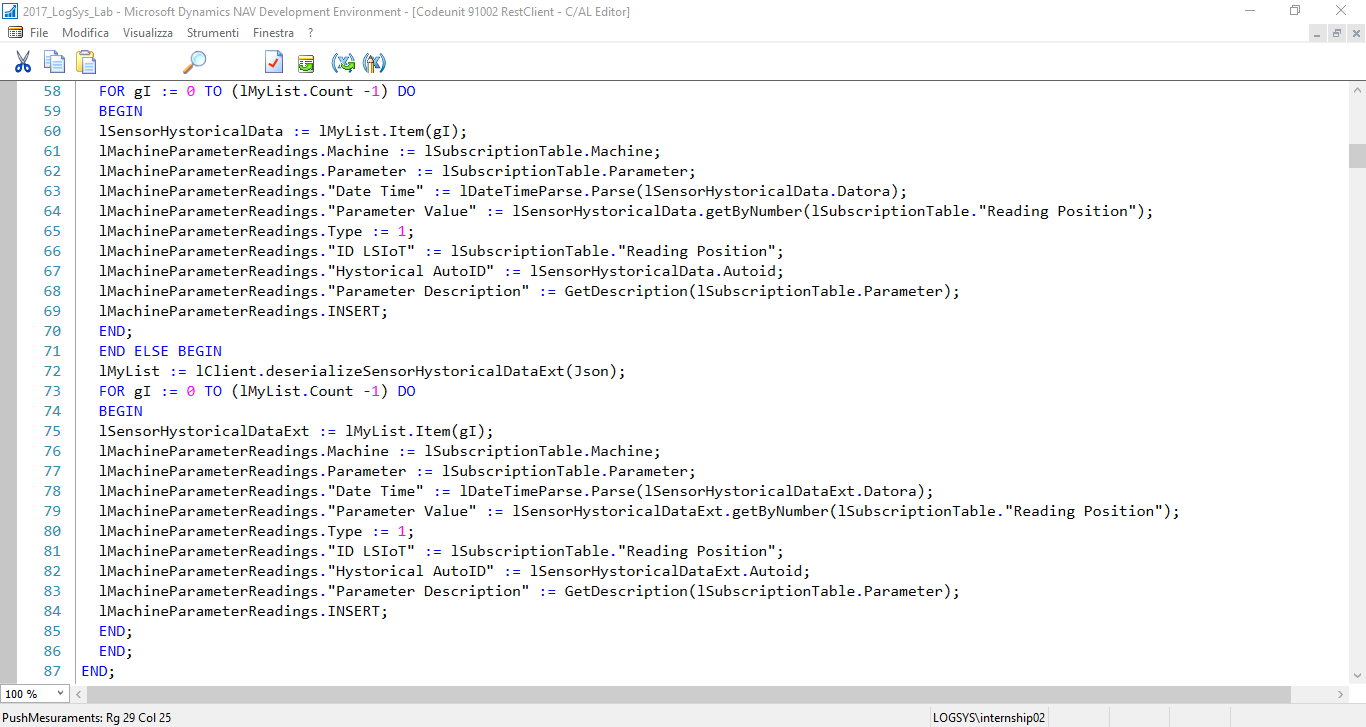
\includegraphics[width=1\textwidth]{images/NAVPushMeasuraments3.png}
%\end{frame}

%\begin{frame}
%\frametitle{Esempio XML}
%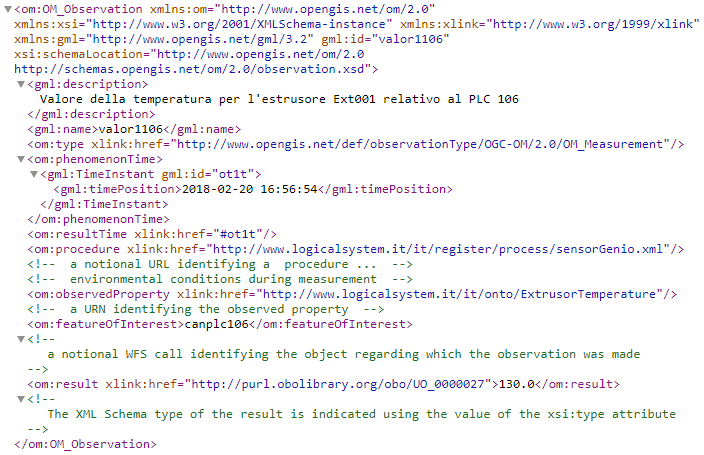
\includegraphics[width=1\textwidth]{images/TemperatureXML2.png}
%\end{frame}

\begin{frame}
\frametitle{Esempio JSON}
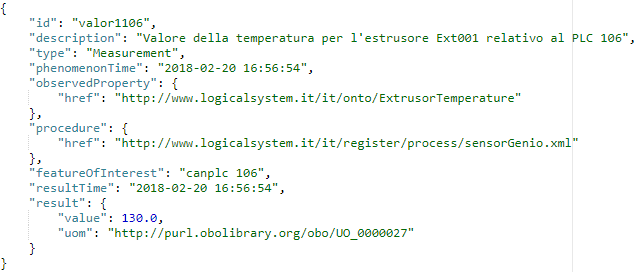
\includegraphics[width=1\textwidth]{images/TemperatureJSON.png}
\end{frame}

%\begin{frame}
%\frametitle{Grafico Misurazioni e misure}
%\begin{figure}%
%	\centering%
%	\subfloat{{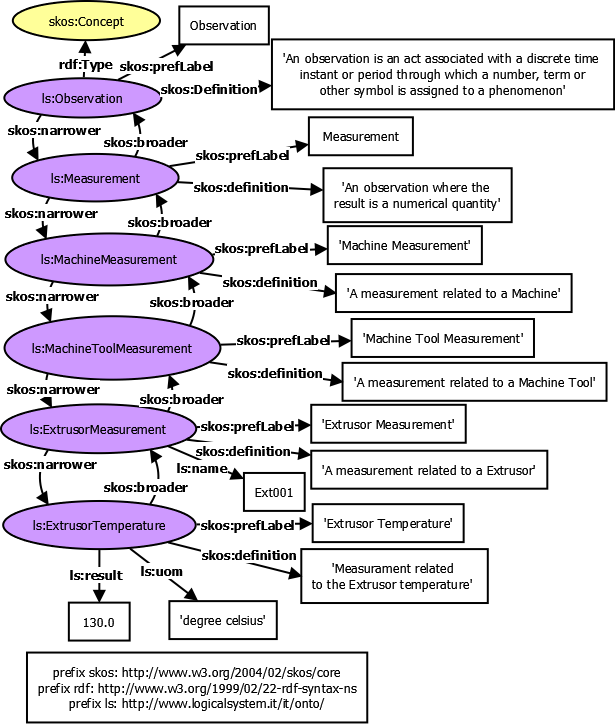
\includegraphics[width=6.84cm]{images/TempExample2.png} }}%
%	\qquad
%	\subfloat{{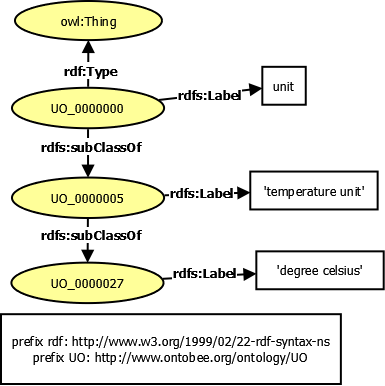
\includegraphics[width=4.7cm]{images/celsius.png} }}%
%
%
%\end{figure}
%\end{frame}

\begin{frame}
\frametitle{Grafico misurazioni e misure}
\begin{figure}%
%\centering
\subfloat{{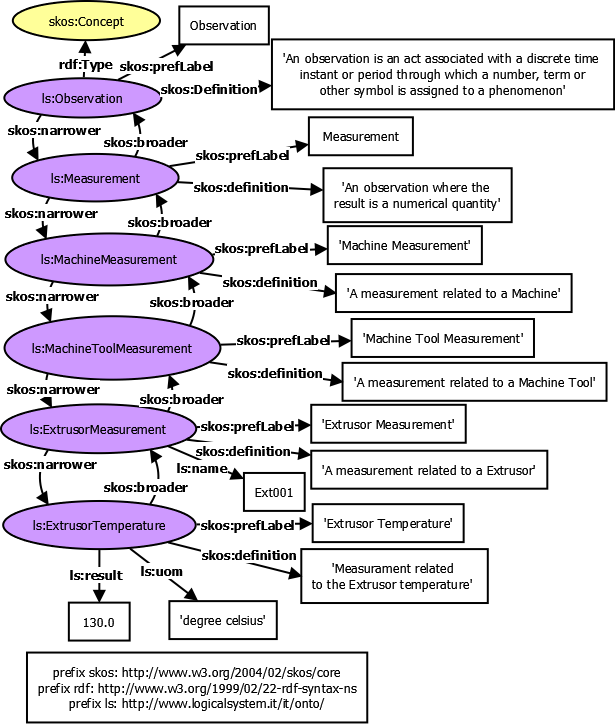
\includegraphics[width=0.565\columnwidth]{images/TempExample2.png} }}%
%\qquad
\hfill
\subfloat{{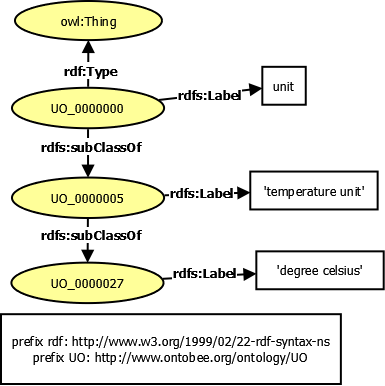
\includegraphics[width=5cm]{images/celsius.png} }}%
%
%
\end{figure}
\end{frame}


%\begin{frame}
%\frametitle{Grafico Misurazioni e misure 2}
%\begin{figure}
%	\subfigure[]{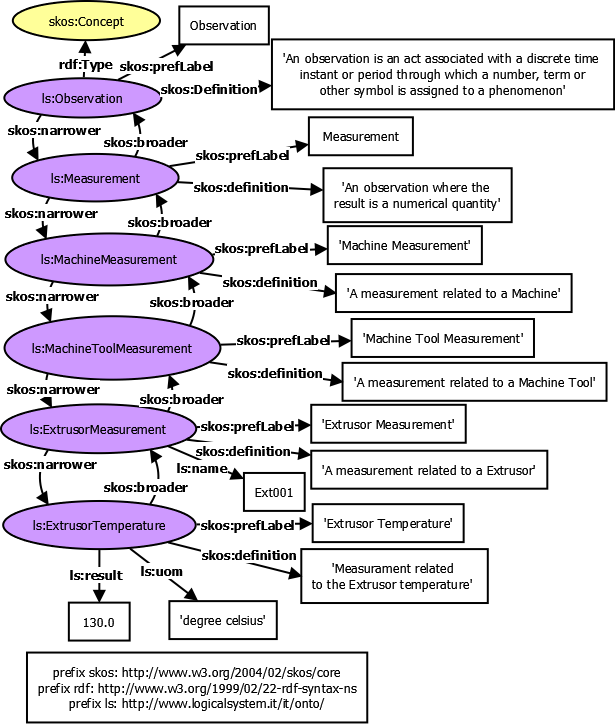
\includegraphics[width=7cm]{images/TempExample2.png}}
%	\hfill
%	\subfigure[]{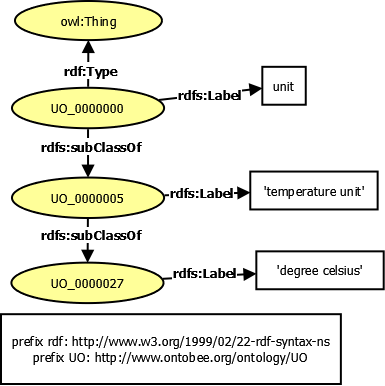
\includegraphics[width=4.7cm]{images/celsius.png}}
%\end{figure}
%\end{frame}

%\begin{frame}
%\frametitle{Grafico Misurazioni}
%\begin{center}
%	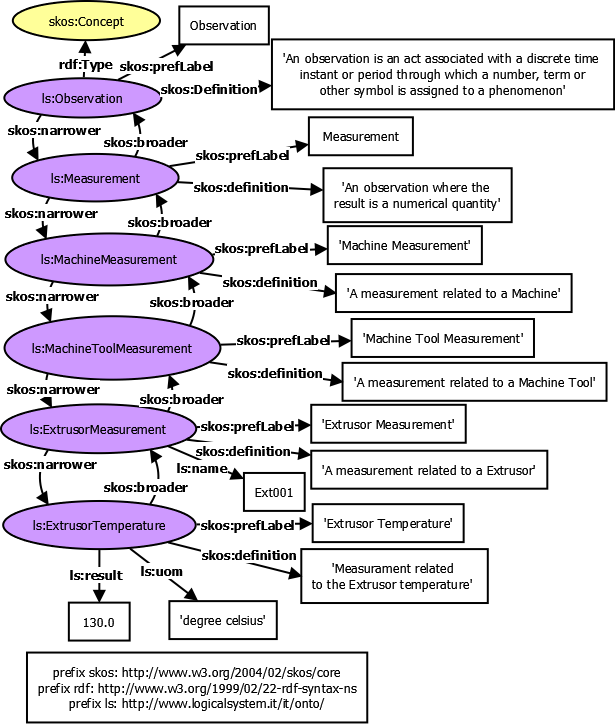
\includegraphics[width=0.6\textwidth]{images/TempExample2.png}
%\end{center}
%\end{frame}

%\begin{frame}
%\frametitle{Grafico Misure}
%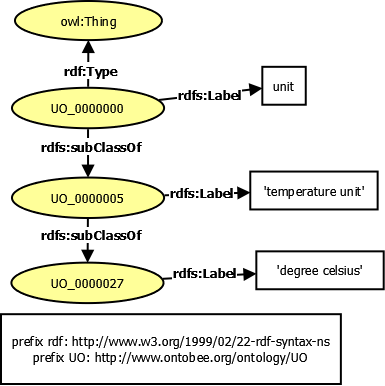
\includegraphics[width=0.6\textwidth]{images/celsius.png}
%\end{frame}

%\begin{frame}
%\frametitle{JSON con annotazione semantica}
%\includegraphics[width=1\textwidth]{images/JSONRestituito.png}
%\end{frame}

\begin{frame}
\frametitle{Conclusioni}
\begin{itemize}
\item L'integrazione tra NAV e la piattaforma ha avuto esito positivo tramite uso del client C\# 
\begin{itemize}
\item Permettendo agli utenti un semplice utilizzo dei servizi
\end{itemize}
%\item Il report PowerBI è disponibile tramite NAV
%\begin{itemize}
%	\item Permettendo agli utenti una visualizzazione grafica dinamica dei dati ricevuti
%\end{itemize}
\item L'ontologia delle misurazioni e delle misure è stata implementata
\begin{itemize}
\item In modo da avere una descrizione dei dati ottenuti dai servizi
\end{itemize}

\end{itemize}	
\end{frame}
\end{document}